\section*{Hardware Implementation}

\section{Schematic v1.0}
\subsection{40-Pin Header for Raspberry Pi 4}

\begin{figure}[h]
    \centering
    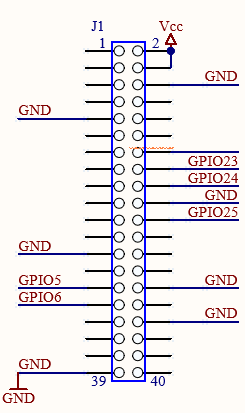
\includegraphics[width=0.3\textwidth]{assets/Stecker}
    \caption{40-pin header designed for the Raspberry Pi 4}
    \label{fig:raspberry_header}
\end{figure}


This connector is a 40-pin header that can be plugged directly onto the GPIO pins of the Raspberry Pi 4.

The design allows the connector to be attached directly to the GPIO header of the Raspberry Pi, saving space and eliminating the need for extra cables. It is also very practical, as the board can be easily removed from the Raspberry Pi 4 at any time.

The Raspberry Pi 4 is powered with 5V. This input voltage is then regulated evenly later on.

\newpage

\subsection{LED Control Circuit for Voice Assistant}

\begin{figure}[h]
\centering
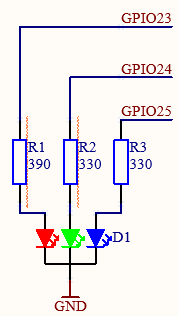
\includegraphics[width=0.25\textwidth]{assets/RGB}
\caption{LED control circuit connected to GPIO pins}
\label{fig:led_circuit}
\end{figure}

In this circuit, an RGB LED is connected to the Raspberry Pi. This LED shows the current status of the voice assistant.

When the voice assistant is turned on, the LED lights up red, indicating that it is active. When one of the buttons is pressed and recording starts, the LED turns blue. If the voice assistant is turned off, the LED stays off.

\subsection*{Circuit Operation}

Each color of the LED is connected to a GPIO pin through its own resistor. These resistors make sure that not too much current flows into the Raspberry Pi or the LED. The red, green, and blue LEDs are connected to GPIO23, GPIO24, and GPIO25. A common cathode RGB LED is used, so it is also connected to ground.

\subsection*{Visual State Indication}

The software on the Raspberry Pi controls the LEDs by setting the GPIO pins to high or low.

This setup provides a clear visual indication of the current mode or function of the voice assistant.m.

\newpage

\subsection{Push-Button Circuit for Voice Assistant}

\begin{figure}[h]
\centering
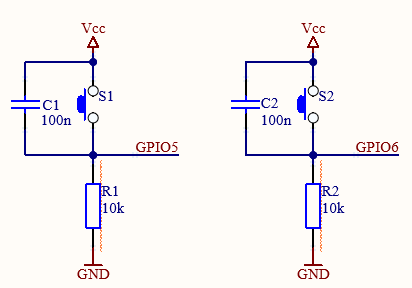
\includegraphics[width=0.7\textwidth]{assets/Schalter}
\caption{Push-button circuits for Record and Toggle functionality}
\label{fig:push_buttons}
\end{figure}

The circuit has two buttons connected to the Raspberry Pi 4. Each button is connected to a specific GPIO pin and controls a function of the voice assistant.
Button S1 is the Record button. When pressed, it starts recording. To stop the recording, you need to press it again.
Button S2 is the Toggle button. This button must be held down continuously to start recording. It is designed specifically for short recordings.
Both buttons have a pull-down resistor, which ensures that the pin stays off (low) when the button is not pressed. In addition, each button has a capacitor to prevent bouncing, which could otherwise cause multiple signals from a single press.

\subsection*{Connection to the Header}
The buttons are directly connected to the 40-pin header of the Raspberry Pi. GPIO5 is connected to S1. GPIO6 is connected to S2

\subsection*{Operation}
When a button is pressed, the corresponding GPIO pin is set to high. The Raspberry Pi detects this signal and performs the desired function.

\newpage

\section{Raspberri Pi 4}

\begin{figure}[h]
\centering
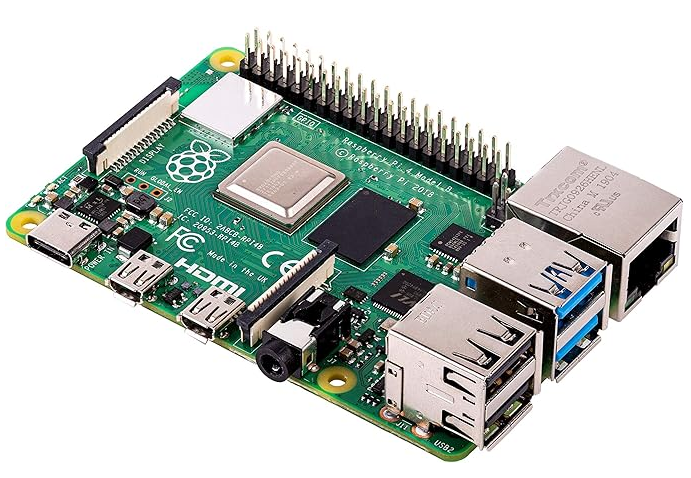
\includegraphics[width=0.6\textwidth]{assets/Raspi.png}
\caption{Raspberry Pi 4}
\label{fig:Raspberry Pi 4}
\end{figure}

A Raspberry Pi 4 with 2GB RAM was chosen. It features a quad-core processor running at up to 1.5GHz and has 2GB of memory. It includes various ports such as USB ports and an Ethernet port. Additionally, the Raspberry Pi has two Micro-HDMI ports, so the display is connected to one of these ports. A microphone is connected via the AUX port for voice recordings. The Raspberry Pi 4 operates at 5V and can draw up to 3A under heavy load. These values represent the absolute maximum ratings.

\newpage

\section{Case v1.0}

\subsection{Custom Enclosure Design for Raspberry Pi 4}

\begin{figure}[h]
\centering
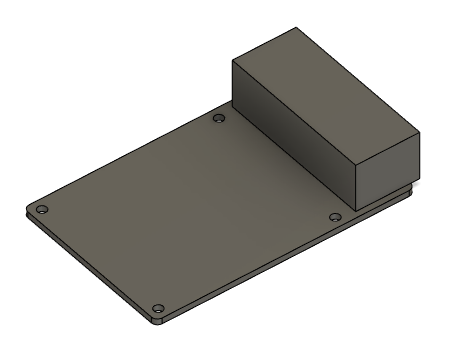
\includegraphics[width=0.6\textwidth]{assets/DG_Raspi4(1)}
\caption{3D Model of the Raspberry Pi 4}
\end{figure}

\subsection*{Introduction}
The Raspberry Pi 4 was modeled at a 1:1 scale to ensure precise fitting and accurate positioning of components.

\subsection*{Design Description}
The Raspberry Pi consists of two main sections: a flat base plate with mounting holes and a raised rectangular area that represents the USB and Ethernet ports of the Raspberry Pi.

The base plate forms the foundation of the Raspberry Pi. The basic structure is a flat, rectangular surface with four screw holes. At the end of the plate, there is a rectangular elevation. This section is intended for the USB and Ethernet ports of the Raspberry Pi and serves as a placeholder for the four USB ports and one Gigabit Ethernet port.

\subsection*{Design Considerations}
The Raspberry Pi 4 was modeled at a 1:1 scale to provide a better understanding of the available space within the enclosure.


\newpage

\subsection{Custom Enclosure}

\begin{figure}[h]
\centering
\includegraphics[width=0.6\textwidth]{assets/DG_Körper_Raspi(1)}
\caption{3D Model of the custom enclosure}
\label{fig:enclosure}
\end{figure}



\subsection*{Introduction}
The Raspberry Pi was used as a reference for the measurements and the positioning of the parts, but it was not included in the printed model. The enclosure was built to be stable and easy to use.

\subsection*{Overall Dimensions}
It is 13cm high, 10cm wide, and 14.8cm long. This size provides enough space for the Raspberry Pi and the circuit board without making the enclosure look too big.

\subsection*{Structural Design}
The body consists of individual parts that are practical both for mounting and for appearance.

\subsubsection*{-Base Structure}
The bottom of the enclosure is a flat, rectangular plate. It serves as the base on which the Raspberry Pi is mounted. There is a slightly raised area on the surface where the Raspberry Pi is screwed in. A rectangular extrusion is included for the USB and Ethernet ports, helping to plan accurate cutouts later. In the center, there is an empty space where the circuit board will be placed.

\subsubsection*{-Side Walls}
The enclosure has four walls. The two side walls are slightly angled backward so that the enclosure stands at a slant, making it easier to view the screen later. On the back side, there is a rectangular cutout for the Raspberry Pi’s USB and HDMI ports. There is also a round cutout for the DC power jack.

\subsubsection*{-Mounting and Reinforcement Features}
At each of the four corners of the base, there are round mounting points for screws. These are fitted with threaded inserts to make it easier to screw and unscrew them later.

\subsection*{Design Considerations}
The Raspberry Pi 4 was modeled in original size to ensure it fits perfectly into the enclosure. The enclosure protects the Raspberry Pi and provides enough space for airflow to prevent overheating. The angled side walls make the enclosure stable and help with mounting the display at a slanted angle later on.


\section{Description of the Enclosure Cover}

\begin{figure}[h]
\centering
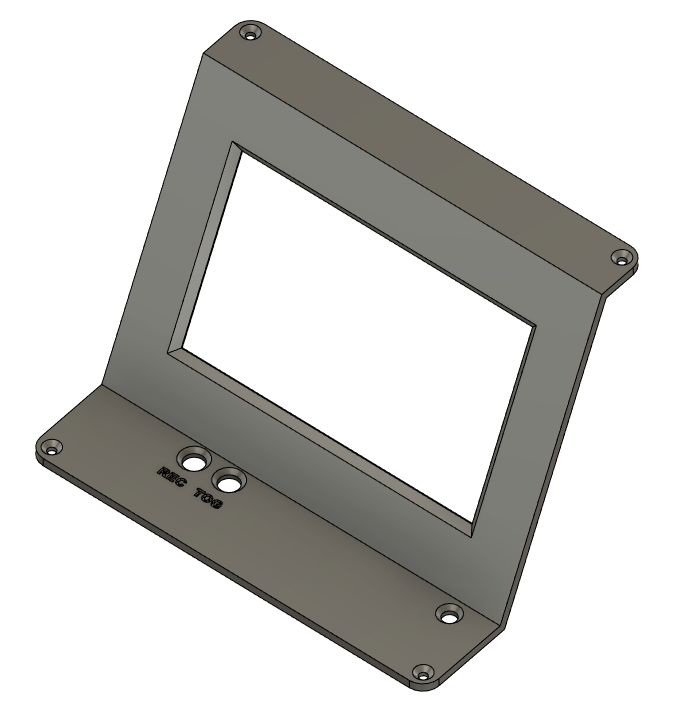
\includegraphics[width=0.8\textwidth]{assets/DG_Deckel(1)}
\caption{3D Model of the enclosure cover}
\label{fig:cover}
\end{figure}

\subsection*{Introduction}
The cover of the case is an important part of the whole setup. It protects the electronics inside and also has important functions. The cover can be firmly attached to the case, but it can also be easily removed. There is a large opening in the cover for a display, and additional holes for buttons and an LED.

\subsubsection*{-) Display Cutout}
At the top of the cover is a large rectangular cutout for the ISR display. It is 11 cm long and 7.5 cm wide, so the display fits perfectly. The edges are rounded to prevent damage to the display.tioning of this window ensures the display remains centered within the user's field of view.

\subsubsection*{-) Button Cutouts}
Below the display, there are two round holes for buttons. One is the record button, which starts a recording. The other is the toggle button. This button must be held down the whole time while speaking into the microphone. The holes are large enough for the buttons to fit in properly and be pressed easily.

\subsubsection*{-) LED Indicator Cutout}
To the right of the buttons, there is a small round hole for an RGB LED. This LED shows the current status of the system – for example, whether it is recording or idle. The LED is placed in a spot where it is clearly visible but does not get in the way.

\subsubsection*{-) Mounting Features}
The cover is designed to be securely attached to the enclosure using four screws. There is a hole for a screw in each corner of the cover, making it easy to screw the cover in place. Threaded inserts are built into the screw holes to ensure the screws hold more firmly.

\newpage

\section{Entire case}

\begin{figure}[h]
    \centering
    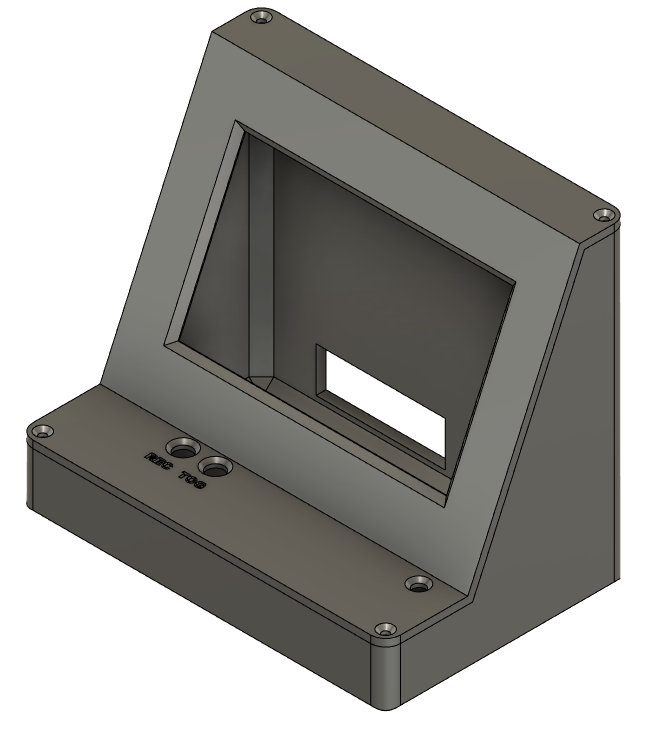
\includegraphics[width=0.7\textwidth]{assets/DG_komplett(1)}
    \caption{3D Model of the entire case}
\end{figure}

\subsection*{Description}

The image shows the complete enclosure. It features a slanted front face with a large rectangular cutout that provides space for a display. Below this cutout are two small circular openings, intended for the toggle button and the record button. The abbreviations for the buttons are also engraved, serving both for orientation and enhancing the appearance.

The enclosure has mounting holes at all four corners on both the top and bottom sides, allowing the cover to be securely attached. The overall design has a rounded style. The edges and corners have been smoothed, both for safety and for aesthetic reasons.

\section{Raspberry Pi 4 Display and Microphone}

\subsection{IPS Display}

\begin{figure}[h]
\centering
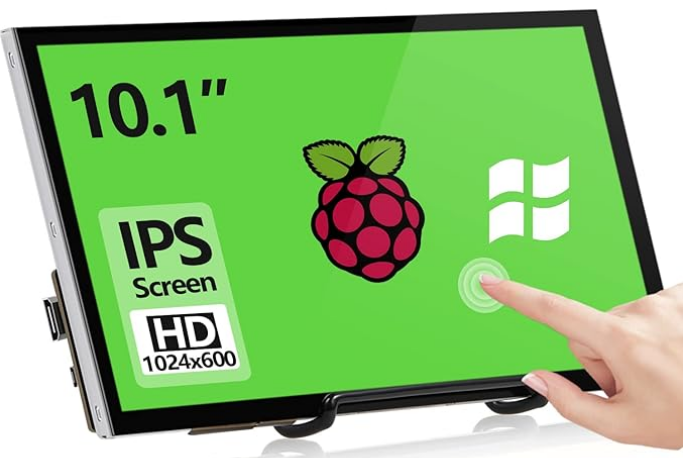
\includegraphics[width=0.7\textwidth]{assets/Bildschirm(1)}
\caption{HAMTYSAN Raspberry Pi Display}
\textcolor{gray}{https://www.berrybase.de/universal-5-0-display-mit-hdmi-eingang-und-resistivem-touchscreen}
\end{figure}

\subsection*{Introduction}
The 10.1-inch IPS touchscreen display is a high-resolution monitor. It was developed for the Raspberry Pi 4 and other compatible devices. It has a resolution of 1024x600 pixels and displays clear images. This allows various outputs and buttons on the screen to be shown more precisely.

\subsection*{Key Features}
The screen has a 16:9 format and a capacitive touchscreen that supports up to five simultaneous touches. This makes operation very accurate and easy. No additional drivers are needed. The connection to the Raspberry Pi is made using an HDMI cable for the video signal and a USB cable for the touch function.

\subsection*{Connection to Raspberry Pi 4}
The connection is made using an HDMI to micro-HDMI cable, which transmits the video. A micro USB cable enables the touch function. This makes the display easy to connect to the Raspberry Pi 4.

\subsection*{Applications}
The display is then used for output. It shows the desired output on the screen. On the display, you can see things like the weather, for example. If no one is speaking into the microphone at the moment, a custom-built page will be shown instead.

\newpage

\subsection{AGPTEK Lavalier Microphone}

\begin{figure}[h]
\centering

\includegraphics[width=0.4\textwidth]{assets/Mikrofon(1)}
\caption{AGPTEK Lavalier Microphone}
\textcolor{gray}{https://www.amazon.de/AGPTEK-Omnidirectional-Kondensator-Transformation-Videokonferenz/}
\label{fig:AGPTEK Microphone}
\end{figure}

\subsection*{Introduction}
The AGPTEK lavalier microphone is a small clip-on microphone. It captures sound from all directions and delivers clear and precise recordings. It works especially well with the Raspberry Pi 4 and other compatible devices.

\subsection*{Functionality}
The microphone is very sensitive and can capture good sound even in noisy environments. It is also very easy to use.

The sound recorded by the microphone is transmitted to the device through the aux port. Once the input reaches the Raspberry Pi, it is sent to the backend. There, the software processes the signal. This software converts the analog signal into digital data. The sound can then be displayed on the screen.


\newpage


\section{Schematic v2.0}

\subsection{Power Supply Circuit}

\begin{figure}[h]
\centering
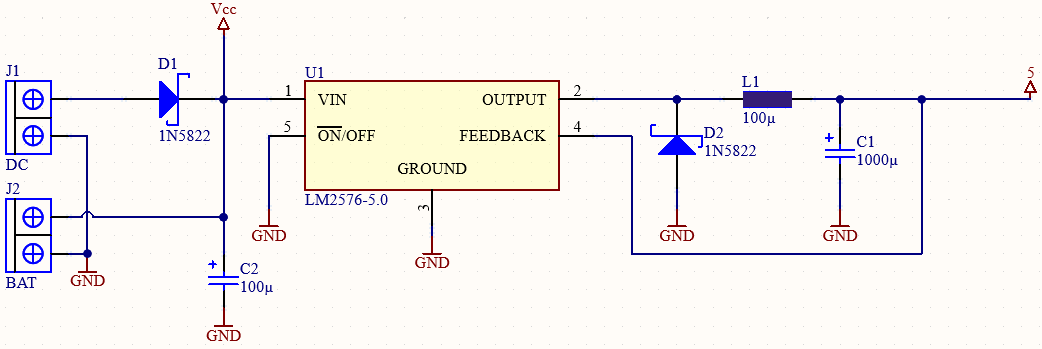
\includegraphics[width=0.9\textwidth]{assets/Power Supply}
\caption{Power supply circuit diagram}
\label{fig:power_circuit}
\end{figure}

\subsubsection*{Introduction}
This circuit was designed to provide a stable 5V power supply, either through a DC input or a 9V battery. The voltage regulation was handled by the LM2576 voltage regulator, which steps down the input voltage to 5V. Later, however, the 9V battery was replaced with two 18650 lithium-ion batteries to improve energy efficiency, increase capacity, and reduce the need for frequent battery replacements.

\subsection{Description 18650 Li-Ion battery}
18650 lithium-ion batteries are small, rechargeable cells with a typical voltage of around 3.7V. When two of them are connected in series, the total voltage is about 7.4V. A Battery Management System (BMS) is added to ensure safe operation of the battery and to prevent issues such as overcharging or deep discharge. In this circuit, the LM2576 voltage regulator converts the 7.4V into a stable 5V output.

\newpage

\subsection{Description LM2576}

\subsubsection{Typical Application}

\begin{figure}[h]
\centering
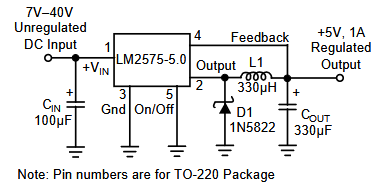
\includegraphics[width=0.6\textwidth]{assets/LM2576 Application.png}
\caption{Typical Application Diagram}
\textcolor{gray}{https://www.ti.com/lit/ds/symlink/lm2576.pdf}
\label{fig:Typical Application Diagram}
\end{figure}

\subsubsection{Description LM2576}
The LM2576 series of monolithic integrated circuits provide
all the active functions for a step-down (buck) switching
regulator. Fixed versions are available with a 3.3V, 5V, or 12V
fixed output. Adjustable versions have an output voltage
range from 1.23V to 37V. Both versions are capable of driving
a 3A load with excellent line and load regulation.
These regulators are simple to use because they require a
minimum number of external components and include internal
frequency compensation and a fixed-frequency oscillator.
The LM2576 series offers a high efficiency replacement for
popular three-terminal adjustable linear regulators. It
substantially reduces the size of the heat sink, and in many
cases no heat sink is required.

\subsubsection{Pinout LM2576}
\begin{figure}[h]
\centering
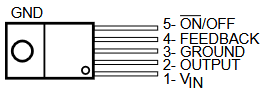
\includegraphics[width=0.6\textwidth]{assets/Pinout.png}
\caption{Pinout LM2576}
\textcolor{gray}{https://www.ti.com/lit/ds/symlink/lm2576.pdf}
\label{fig:Pinout LM2576}
\end{figure}

\subsection{Circuit Description}
\subsubsection*{Power Input}
The circuit has two options for power supply: a DC jack connector named J1 for an external power source, and a battery connector named J2 for two lithium-ion 18650 batteries connected in series. The Battery Management System (BMS) is mounted directly on the lithium-ion batteries. To prevent current from flowing between the two sources, a Zener diode is used. Capacitor C1 helps stabilize the input voltage.

\subsubsection*{Voltage Regulation}
The LM2576 voltage regulator converts the input voltage into a stable 5-volt output. The VIN pin receives the input voltage. Pin 3 is connected to ground. Pin 5 is the ON/OFF control pin, which is connected to ground to enable the regulator. Pin 2 provides the regulated 5 volts.

\subsubsection*{Output Stage}
To make the 5-volt output as smooth as possible, it is stabilized with an inductor. The Schottky diode D3 prevents current from flowing back into the circuit. Capacitor C2 further reduces voltage fluctuations.

\subsection*{Conclusion}
Originally, the circuit was designed to run on a 9-volt battery. However, it was replaced with two 18650 lithium-ion batteries. This solution is more efficient, has a higher capacity, and is more effective overall. The circuit can still be powered by an external power source and reliably delivers a stable 5-volt output.

\newpage

\section{Battery-powered supply}

\subsection{BMS 2S Li-Ion Battery Pack}

\begin{figure}[h]
\centering
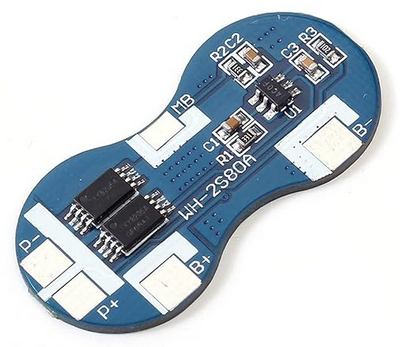
\includegraphics[width=0.5\textwidth]{assets/BMS}
\caption{DollaTek 3Pcs 2S Li-Ion BMS}
\textcolor{gray}{https://www.amazon.de/DollaTek-Ladegeraet-Schutzplatine-Ueberladung-Ueberentladungsschutz}
\label{fig:BMS}
\end{figure}

\subsection*{Introduction}
\noindent This Battery Management System is specifically designed for two 18650 lithium-ion battery cells connected in series. This results in a typical voltage of about 7.4V. The BMS includes a special IC that constantly monitors important values such as voltage, current, and temperature. This ensures safe operation and extends the battery's lifespan.

\subsection*{Key Functionalities}
The BMS performs many protection functions. It checks each cell individually to make sure the voltage does not get too high or too low. If the current becomes too high or too low, the BMS shuts off the battery to prevent damage or overheating. The temperature is also monitored: if it gets too hot, the BMS disconnects the circuit to prevent dangerous situations like a fire.

\subsection*{Protection Mechanisms}
The system also protects the battery from overcharging by stopping the charging process once a certain maximum voltage is reached. In case of deep discharge, it stops discharging to prevent damage to the cells. If a short circuit or sudden high current is detected, the BMS immediately disconnects the battery to protect it.

\subsection*{Balancing and Cell Equalization}
In a 2S configuration, it's important that both cells are charged evenly. The BMS includes a balancer that equalizes the voltage between the cells so both charge to the same level. This improves performance and increases the battery pack’s lifespan.

\subsection*{Detailed MOSFET Operation}
An important part of the BMS are the MOSFETs. These act as electronic switches and control the flow of current between the battery and the device or charger.

\subsection*{Operational Details}
Under normal conditions, the MOSFETs are turned on and allow current to pass. But if the BMS detects an error—such as overcharging or a short circuit—it switches the MOSFETs off. This breaks the circuit and protects the battery. Once everything is back to normal, the BMS turns the connection back on.

This modern BMS reliably protects the battery, keeps cell voltage balanced, and reacts quickly to problems. This makes the battery safer and helps it last longer.

\newpage

\section{PCB Design}

\subsection{Top-Layer}

\begin{figure}[ht]
    \centering
    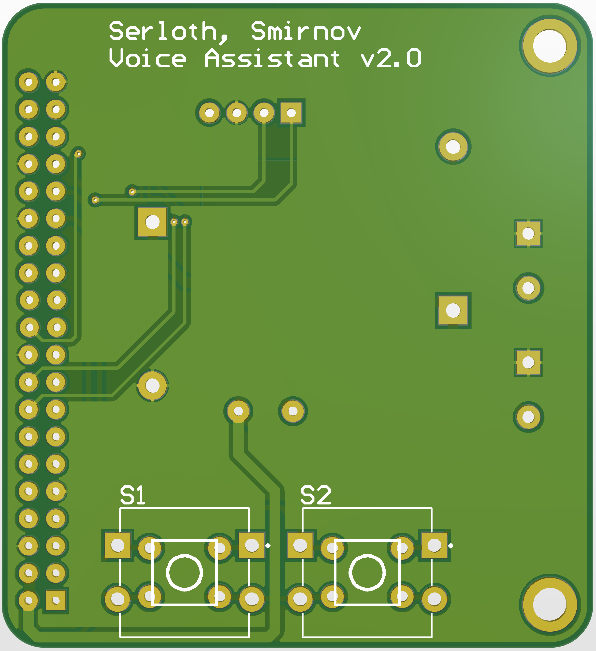
\includegraphics[width=0.5\textwidth]{assets/TopLayer}
    \caption{Top-Layer}
    \label{fig:top-layer}
\end{figure}

\subsection*{Description Top-Layer}
On the top layer of the PCB, there are two push buttons. The left button is the 'Record' button, and the right button is the 'Toggle' button. They have been placed so that they end up in the center of the enclosure, providing sufficient space to press them comfortably. The enclosure was then designed with two recesses that allow the buttons to protrude through, ensuring easy access for the user.

\newpage

\subsection{Bottom-Layer}

\begin{figure}[ht]
    \centering
    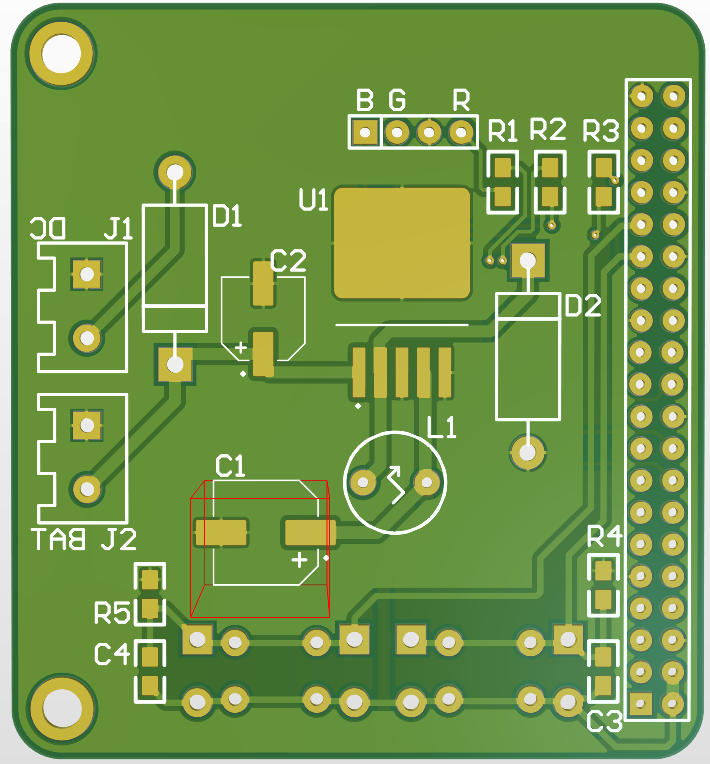
\includegraphics[width=0.5\textwidth]{assets/Bottom Layer.png}
    \caption{Bottom-Layer}
    \label{fig:bottom-layer}
\end{figure}


\subsection*{Description Bottom-Layer}
All the important components for power supply and other functions are placed on the bottom side of the circuit board.
The LM2576 is a voltage regulator that takes a higher input voltage and converts it into a lower, stable output voltage. It is placed near the power input connectors so that the power paths stay short. The large 20x20 header connects the board directly to the Raspberry Pi 4, providing a strong mechanical and electrical connection.
There are two small 2-pin headers for power input: one for connecting a Li-Ion battery, and one for a DC jack (power adapter). This allows the system to be powered by either a battery or an external power supply. There is also a 4-pin header for connecting an RGB LED. The LED is mounted at the top of the enclosure and connected via a cable, while the control electronics stay on the bottom side of the board.
Two diodes are included in the power paths to control the flow of current from the battery or the DC jack to the voltage regulator. They also protect against reverse polarity or backflow of current. An inductor works together with the LM2576 to convert the voltage. It temporarily stores energy and is sized based on the needed output power.
Capacitors are used to stabilize the voltage at both the input and output of the voltage regulator. The capacitor shown in the circuit diagram is especially important for the output side. It must have sufficient capacitance and an appropriate voltage rating. Resistors R1, R2, and R3 serve as current-limiting resistors for the LED. Resistors R4 and R5 are used as pull-down resistors.
Placing these components on the underside has the advantage of freeing up space on the top side for mechanical parts. Splitting the layout across two layers also allows for a more compact design.


\section{Case v2.0}

\begin{figure}[htbp]
    \centering
    \begin{minipage}{0.45\textwidth}
        \centering
        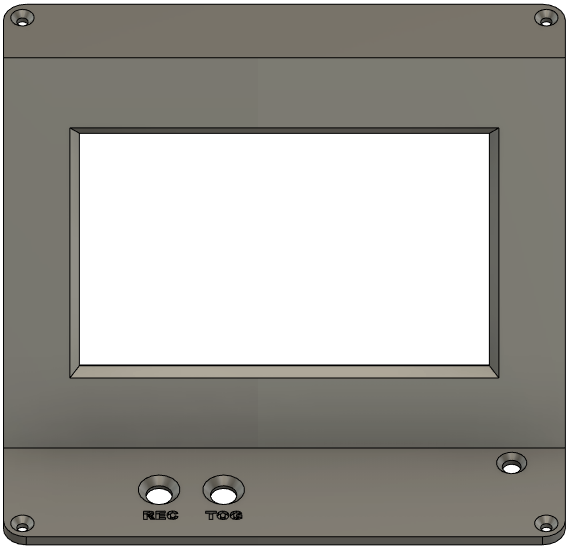
\includegraphics[width=\textwidth]{assets/Deckel v2.0 front.png}
        \caption{Case v2.0 front}
        \label{fig:case_v2_front}
    \end{minipage}
    \hfill
    \begin{minipage}{0.45\textwidth}
        \centering
        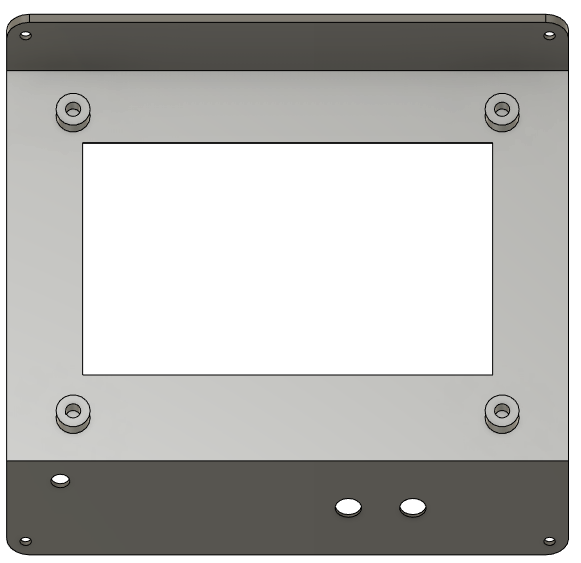
\includegraphics[width=\textwidth]{assets/Deckel v2.0_Rueckseite.png}
        \caption{Case v2.0 back}
        \label{fig:case_v2_back}
    \end{minipage}
\end{figure}

\subsection*{Changes}

Due to inaccurate measurements, the display could not be properly mounted into the housing. The measurements have now been revised to ensure that the opening in the housing is large enough for the screen and that the screw holes align precisely with those of the display.

Additionally, the buttons have been reworked. Since their positions were adjusted in PCB version 2.0, the corresponding button openings in the housing were moved further inward. As a result, the buttons can now be easily pressed through the newly adjusted openings.